\documentclass[11pt, letterpaper]{article}

\usepackage[margin=1in]{geometry}
\usepackage{graphicx}
\usepackage{hyperref}
\usepackage{authblk}
\usepackage{float}
\usepackage{amsmath, amssymb}
\graphicspath{{./images/}}
\usepackage{biblatex}
\usepackage{titling}
\addbibresource{./PNNL-CT.bib}

\title{A Quantitative Analysis of Industrial Computed Tomography}
\author {Thomas Pasfield}
\author{Kian Greene}
\author{Dylan Pereira}
\author{Ryan Reynolds}
\author{Ioannis Paraschos}
\affil{Embry-Riddle Aeronautical University, Daytona Beach, FL}

\begin{document}
\begin{titlingpage}
    \maketitle

    \vfill

    \begin{abstract}
        Additive manufacturing (3D printing) is increasingly utilized within modern industry. 3D-printed components introduce new structural behavior and problems to account for. Computed Tomography (CT) provides a method to analyze this structure without compromising the material, making it a valuable tool moving forward. This work aims to consolidate analysis methods to improve their usefulness within the additive manufacturing industrial process. Existing methods and modified approaches are tested on a 1789-image dataset provided by the Pacific Northwest National Laboratory. Our analysis focuses on segmentation, dimensioning, and 3D-printing-specific needs such as layer separation, in-fill analysis, and path accuracy. We approach segmentation via region-growing methods, where the user provides seed values. Our various dimensioning implementations utilize optimization and voting methods to fit prior knowledge about shape to the observed article. 3D-printing-specific features build from our other methods to observe in-fill density and layer separation. Evaluation methods are employed to provide quantitative analysis of scanned samples. This work hopes to aid in standardizing and certifying CT analysis within the additive manufacturing industrial field.
    \end{abstract}
\end{titlingpage}

\section{Introduction}
\subsection{Industrial Partner}
    The Pacific Northwest National Laboratory (PNNL) is a U.S. Department of Energy research lab that specializes in nuclear and material science. They have been located in Richland, WA, since the lab's inception in 1965. Over the decades, they have diversified from nuclear weapons research to medicine, biology, environmental science, and more.\cite{noauthor_national_nodate} To improve industry support for additive manufacturing in precision applications, the lab wishes to explore applying computed tomography to the task.

\subsection{Computed Tomography}
    Computed Tomography is much better known by the names of CT or CAT scans. Tomography refers to imaging a sample with a penetrating wave to view the density. If you have ever held an object up to a light to see inside it or through it, you have performed tomography. The name "Computed Tomography" comes from the complex computational process that allows a 3D volume to be reconstructed from tomographic images at different positions.

    In CT, imaging is performed iteratively. Once the sample is placed into the machine, X-ray images are taken at various angles about one axis around it. These images are processed via the Radon Transform in order create a 3D volume. The resulting reconstruction is higher quality if finer angle differences are used. The volume is stored as a third rank tensor, with each element referred to as a "voxel."

\subsection{Provided Data}
    For this work, PNNL provided a processed volume of an additively manufactured test object. This test object, seen in Figure \ref{fig:test-object}, consists of three distinct regions and materials. The lower region was printed in a Polylactic Acid (PLA) filament, the middle region was printed with a Polycarbonate (PC) filament, and the upper region was printed with a nylon filament. Each region is printed with an angled planar boundary between them at $26.57^\circ$ from horizontal. The print was prepared with a standard grid infill pattern at 95\% infill density.

    \begin{figure}[H]
        \centering
        \label{fig:test-object}
        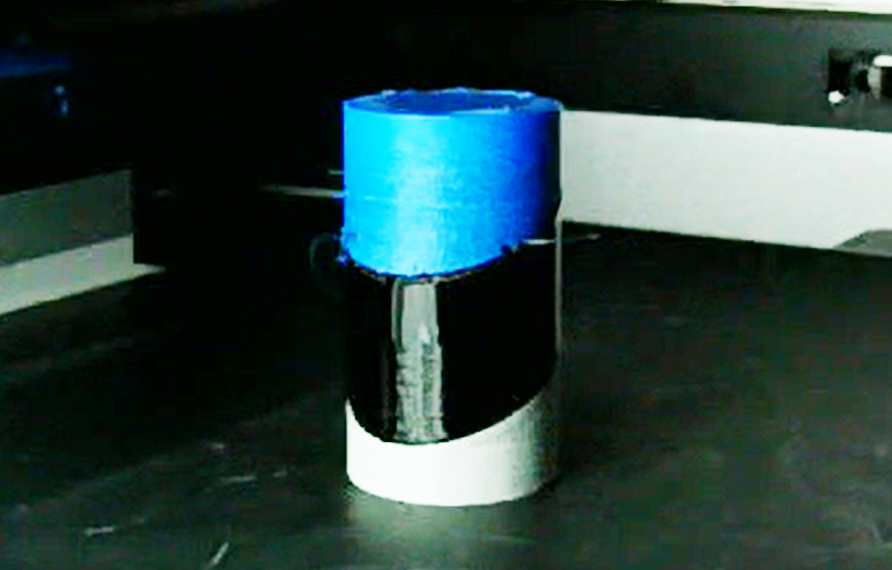
\includegraphics[width=0.75\textwidth]{test_sample.png}
        \caption{\emph{An image of the test sample immediately after printing, as taken by a remote-monitoring camera mounted to the printer. Provided by PNNL.}}
    \end{figure}

    The CT scan was conducted by PNNL and is known to have consisted of several thousand individual images. The exact count was not provided. The Radon transform, and all relevant post-processing was conducted prior to the delivery of the data to our team. The resulting volume was stored as 1789 individual TIFF images. The images are uncompressed, grayscale, and stored with single-precision floating point values. Each image is $1085 \times 1085$ pixels in resolution. When assembled into the full volume, the resulting tensor has dimensions of $1085\times1085\times1789$. Each voxel has a 1:1:1 aspect ratio and a scale of 20.4382 $\mu$m.
    
    At full precision, storage of this tensor takes about 8.4 GB of RAM. For easier processing by team members, the tensor was normalized and precision was reduced to unsigned 8-bit integer values. This is acceptable as our data is relative to itself and does not represent any exact physical unit.

\subsection{Scope of the Problem}
    Additive manufacturing (AM) presents a unique set of challenges when it comes to structural integrity. In plastic AM, print quality can depend on many qualities such as the extrusion rate, print speed, extruder temperature, print-bed temperature, and the filament itself. These can all affect the outcome of the print and can lead to defects and weaknesses within the component. Even without these defects, the structural behavior of a print is difficult to simulate due to complex and non-uniform internal geometries. In metal AM, similar issues arise, as well as the addition of cavitation and bubbling within the metal. Resin AM has much more consistent print characteristics, but lacks the flexibility of other methods.

    To address these problems within AM, we have analyzed a CT scan of a test sample provided by PNNL. We have determined three suitable approaches for gathering useful and actionable data related to the print. These three approaches are dimensioning, segmentation, and infill analysis.

    \emph{Dimensioning.} Dimensioning refers to the quantification of the size of the object and its features. In the case of our sample, it includes the diameter of the cylinder, its height, the heights of each region, the size of interior defects, and other such features. Dimensioning helps to characterize printer performance and accuracy.

    \emph{Segmentation.} Segmentation is the separation of an image into distinct similar regions. In the case of CT scans of 3-D prints, the goal is to segment each print material so that it can be analyzed through other methods independently.

    \emph{Infill Analysis.} Infill Analysis involves quantifying properties of the printing process. Our primary goal of this analysis is to quantify the infill density observed so that it can be compared to the settings configured the slicing software used to prepare the model for printing.

\section{Methodology}
\subsection{Dimensioning}
    Dimensioning was separated into two primary tasks for this test article. As the sample print was a cylinder, we focused on specific methods for analyzing the diameter and the height throughout locations on the object. Third-party tools were explored for general purpose measurement at arbitrary locations and shapes.

    \subsubsection{Circle Masking}
        As the first approach we attempted, we expected it to be too naive of a solution. It relies on assuming that measuring the diameter is more complex than just measuring along the x and y axes of the image. Knowing this, we must find a way to approach the measurement from all angles. Lacking any other ideas, we took the simple approach of comparing the cross-section to a known circle that we define.

        The first step of this process is to perform an edge detection on the circular cross-section. We have used the Canny Edge Detector method built in to OpenCV\cite{opencv_library}. This method accepts several inputs, but the important ones to this process are the two threshold values used in the double thresholding the method performs. These are chosen by pure guesswork, indicating that this method may be unsuitable for future use. The final values decided upon were \verb|threshold1=500| and \verb|threshold2=500|.

        Once the edges have been detected, we now need a circle to compare it with. OpenCV is once again used to draw this circle into a matrix. We can provide the radius and center coordinates as integer inputs. This has a predictable limitation of only supporting diameters of an even number of pixels, and not supporting center locations that don't perfectly align with the pixel grid. The two images are seen in Figure \ref{fig:edges-v-circle}.

        The two images are compared using an element-wise logical AND operation. This results in a matrix containing ones only where the two images perfectly overlaps. Maximizing the sum of the image results in the best fit circle. The SciPy\cite{virtanen_scipy_2020} Python library is used to perform multi-variable optimization to automate the fitting process.
        \begin{figure}[H]
            \centering
            \label{fig:edges-v-circle}
            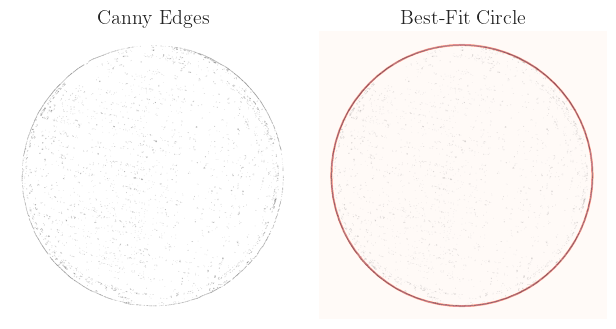
\includegraphics[width=0.75\textwidth]{edges_v_circle.png}
            \caption{\emph{A comparison of the edges detected on a circular cross-section to the best fit circle that matches.}}
        \end{figure}


    \subsubsection{Hough Circle Transform}
        Another method used to approach dimensioning was the use of OpenCV's \verb|HoughCircles| function \cite{noauthor_opencv:_nodate}. This was used in conjunction with the Canny edge detection method to fit a circle onto the outer rim of a slice. From this outer circle, the radius, and thus the diameter, was estimated.

        After the image slice was read, it was put through a median blur operation to reduce noise while keeping edge information for the Canny edge detection. Then, the \verb|HoughCircles| function was used on the results of the edge detection, which employs the Hough transform through the use of the Hough gradient method. An output image was then generated which overlaid the circle(s) onto the input image slice.

        A potential caveat with this method was the number of false positives that occurred due to the "cross-hatch" pattern of the material infill within the image slice itself. However, this seems to have been remedied by implementing the Canny edge detection first, but further study may be performed into this issue.

        \begin{figure}[H]
            \centering
            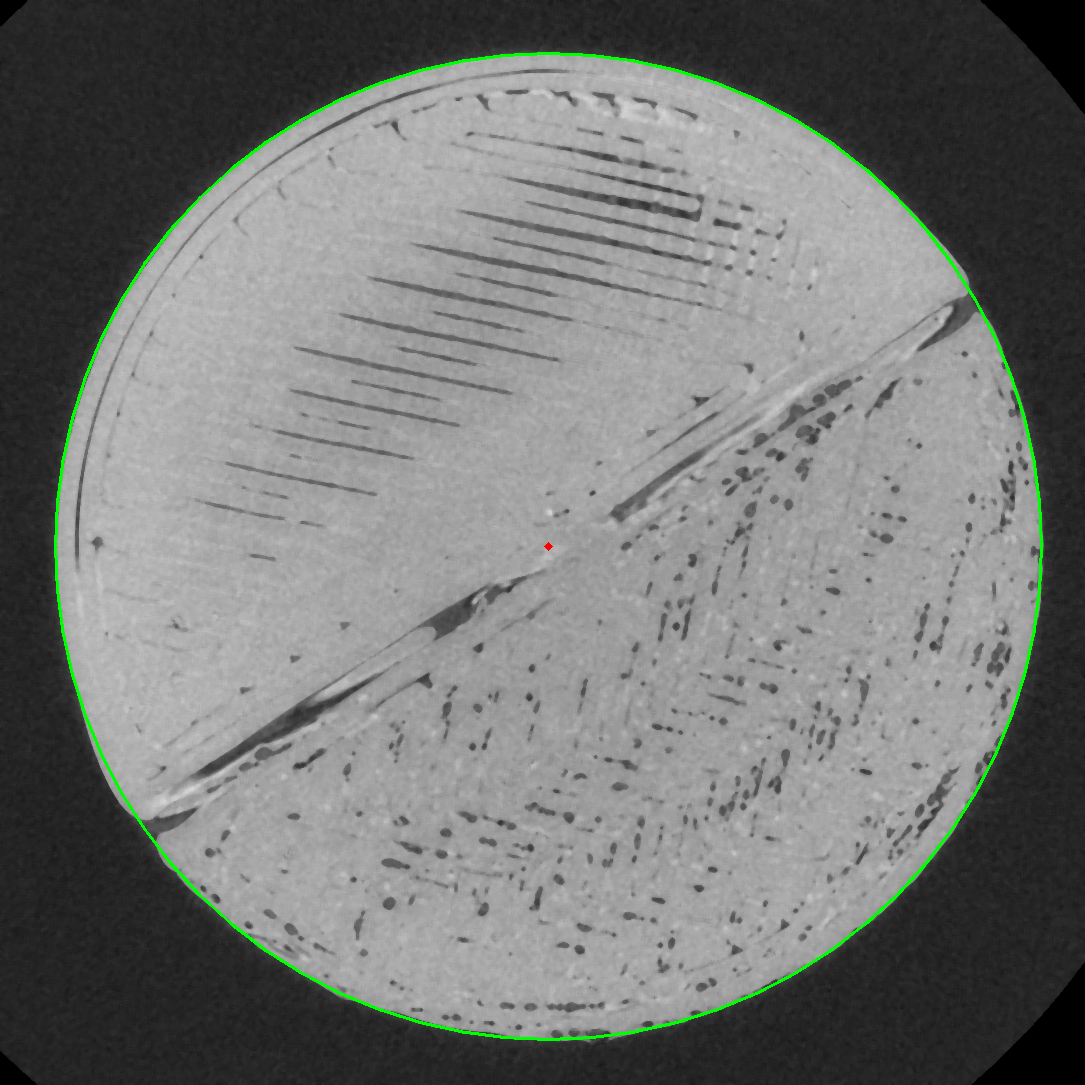
\includegraphics[width=0.5\textwidth]{HoughCirclesTest.PNG}
            \caption{\emph{An example output image of the} HoughCircles \emph{method, where the radii were constrained between 450 and 500 pixels so as to only detect the outer edge of the slice.}}
            \label{fig:HCT}
        \end{figure}
           
        Another remedy to this was the selection of initial guesses for inner and outer pixel radii of the image. The \verb|HoughCircles| function requires a minimum and maximum radius limit in its input parameters, and designating these as 450 pixels and 500 pixels, respectively made it so that only the outer rim circle was detected, displayed in Figure \ref{fig:HCT}.

    \subsubsection{Height Thresholding}
    Height dimensioning was handled via a very simple approach of thresholding the image to ignore background values, then determining the first pixels on the top and the bottom of the sample which exceeded that threshold. Simply finding the difference between the two pixels allowed for easy height measurement.

    \subsubsection{3D Slicer}
    Knowing that the previously discussed methods are very limited to just our test article, we wanted to pursue a more general purpose method of dimensioning. We found an open-source tool named 3D Slicer that allows for both easier overall measurement, and measurement of a wider range of features. Its user interface is seen in Figure \ref{fig:3DSlicerEx}

    3D Slicer was created for medical applications for viewing CT scans and MRIs. It supports a wide range of data formats, as well as supporting the voxel scale in all outputs. It is intuitive to use and allows us to measure a feature by simply clicking and dragging the mouse pointer. It also supports curves in a similar manner.

    \begin{figure}[H]
        \centering
        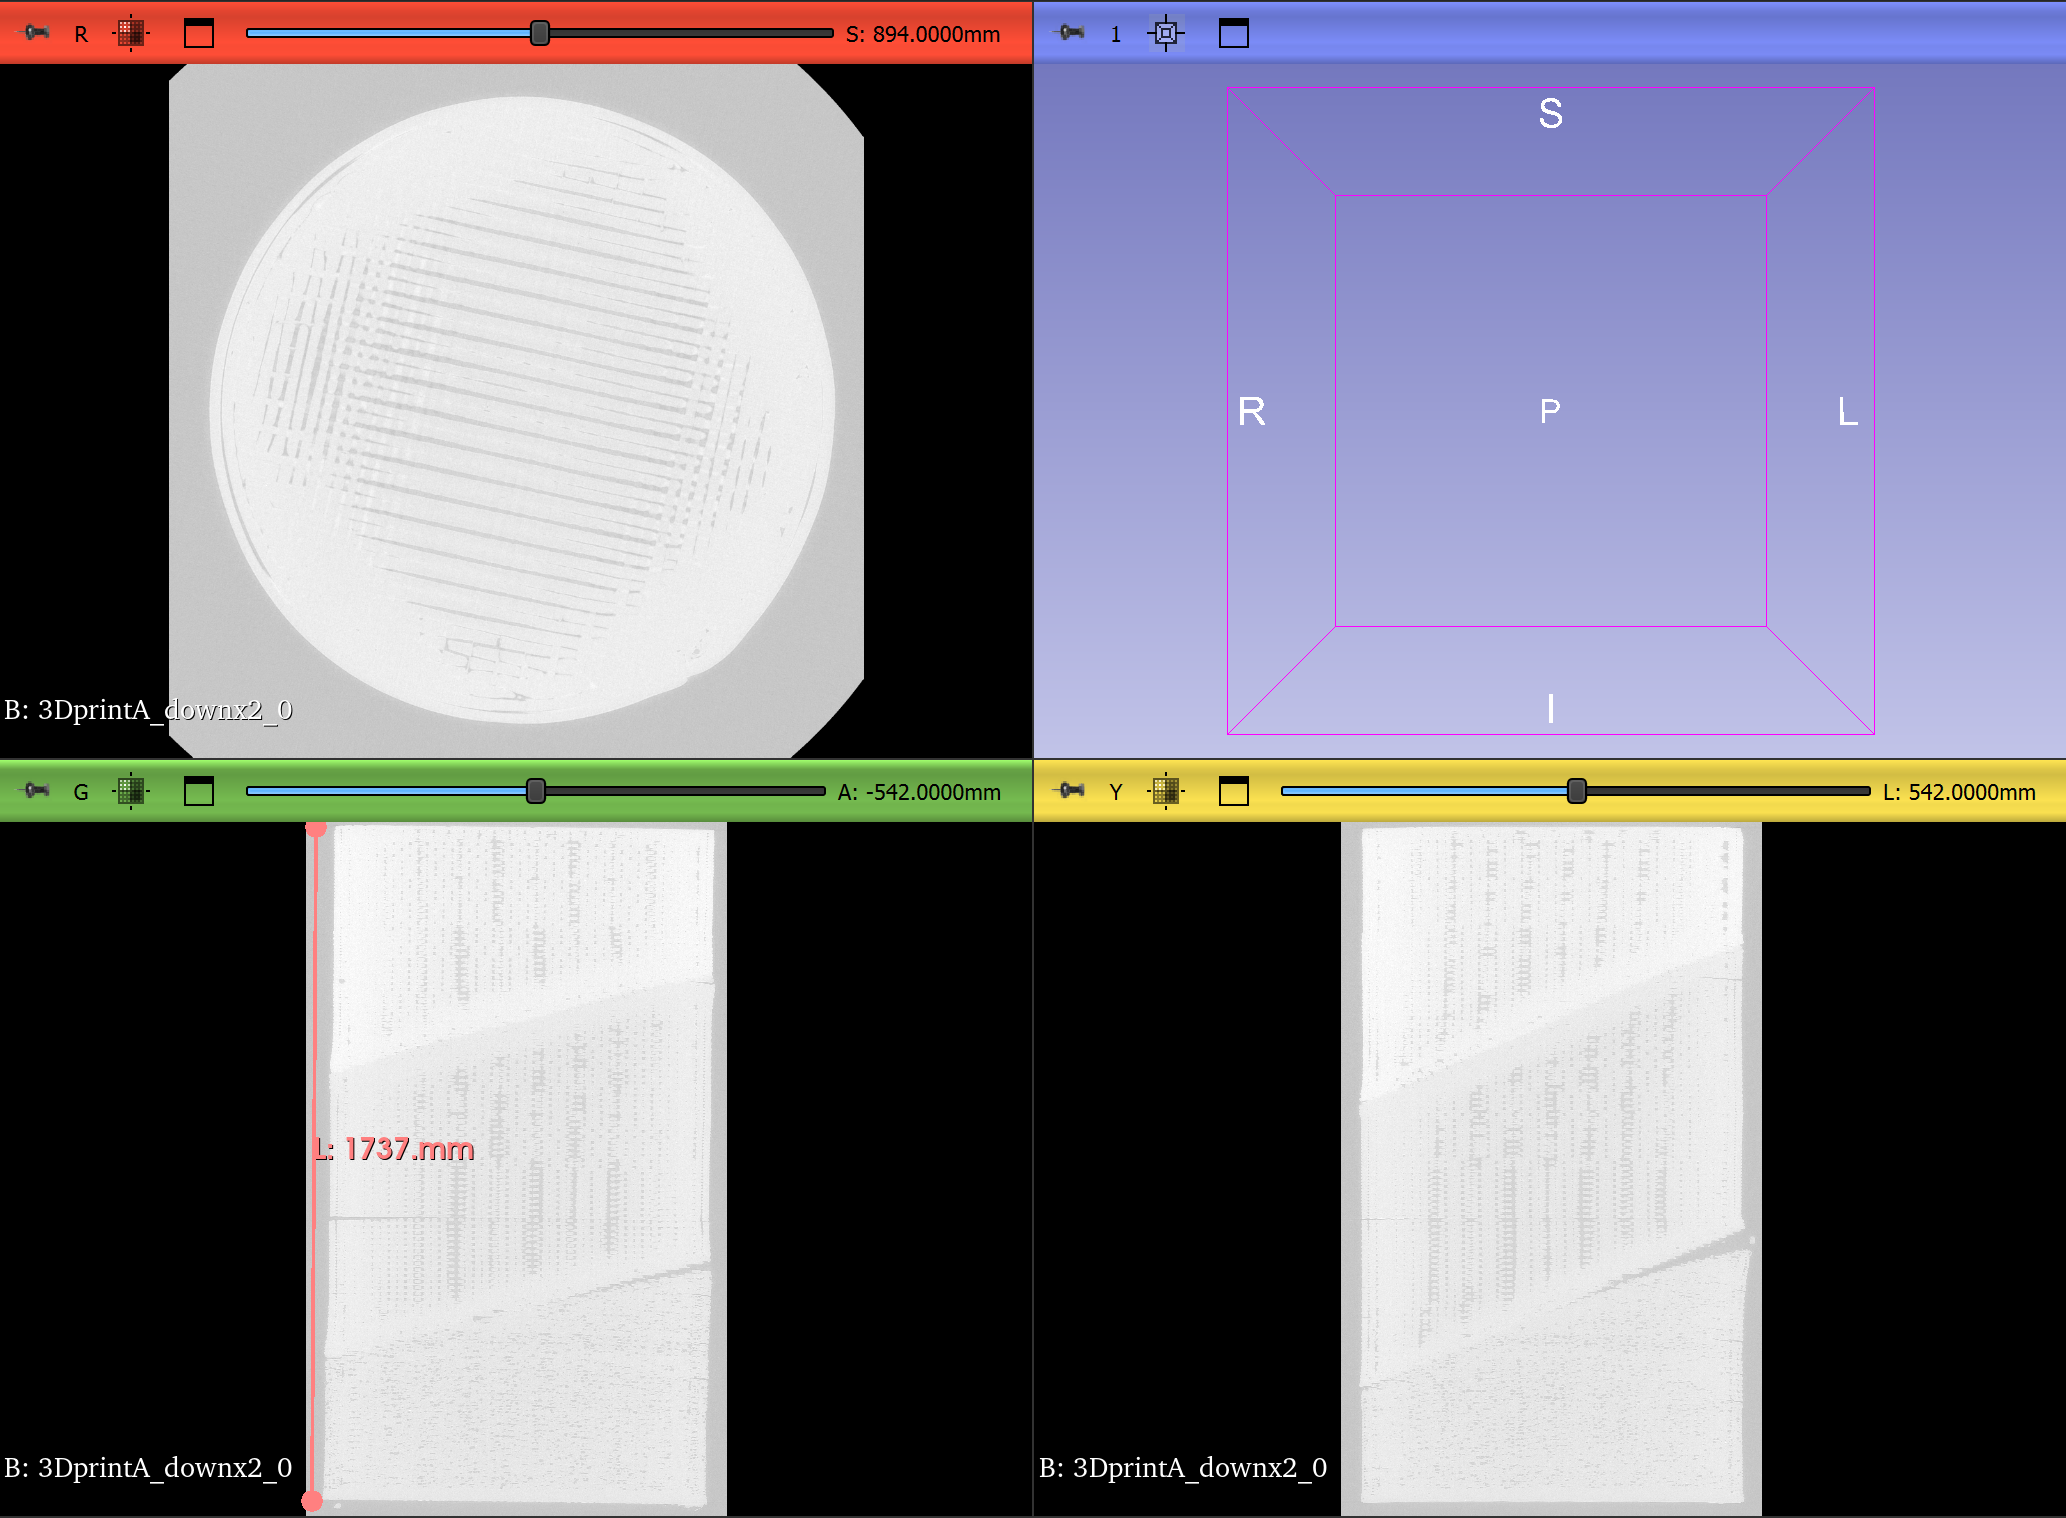
\includegraphics[width=\textwidth]{3D_Slicer_Example_Image.png}
        \caption{\emph{Example of the 3D Slicer object viewer layout. The orange line in the lower left panel displays an approximate height measurement in pixels, incorrectly labeled with units of millimeters.}}
        \label{fig:3DSlicerEx}
    \end{figure}

\subsection{Infill Analysis}
    \subsubsection{Grid Subdivision}
    This first approach features varying layers of precision: Using a grayscale version of a particular slice, a threshold value is input by the user, and pixels darker than the threshold are considered air pockets, while pixels lighter than the threshold are treated as part of the material.  This strict binary is applied to the entire target slice to create a black-and-white-only image from the original grayscale image, as seen in the following figure:

    \begin{figure}[H]
        \centering
        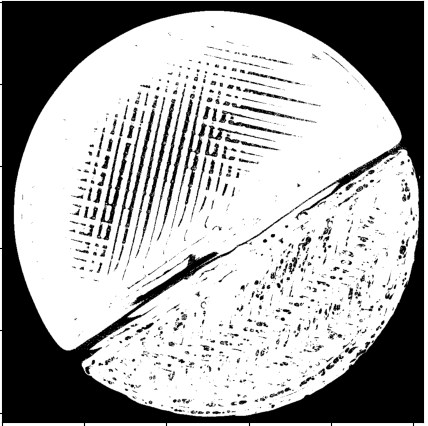
\includegraphics[width=0.5\textwidth]{images/575blackwhite.png}
        \caption{\textit{Example of Image Slice 575, upon which a threshold value of 100 was applied to divide material from air in the slice.  Any pixel with a value above 100 is considered "material", while pixels below 100 are treated as "air".}}
        \label{fig:575blackwhite}
    \end{figure}

    Next, the target slice is subdivided into a grid of smaller regions based on a grid-scale value also provided via user input.  Within each region of the grid, a ratio of material to air is calculated, and a colormap of ratios across the regions of the target slice is created, with a different color dependent on each region's material-to-air ratio.  Additionally, by varying the scale of the grid, heatmaps of various resolutions can be created, which reveals patterns in the deposition of each material in the object.

    \subsubsection{Region-Filling}
    Our second approach consists of isolating regions of the cross-sections, finding their edges, closing gaps within those edges, and filling the form back in to find the area without holes. This area without holes can be compared to the actual observation in order to determine the infill density. This method shows a lot of promise on more generalized datasets as it is not dependent on the assumption that the test article is a cylinder.

    \subsubsection{Mask Comparison}
    This third approach seeks to build from the work done by other members. The dimensioning work provides known diameters and center locations for each cross-section. This can easily be adapted into a 100\% filled area for each cross-section.

    The observed cross-section is first prepared by thresholding in order to remove all background values so that they do not affect the summation. A mask is created from the known diameter data, and the mask is scaled by the mean of intensities for the cross-section material. The sums of these images are compared in order to estimate an infill density. The comparison of the observed image and the mask is shown in Figure \ref{fig:circle-mask}.

    \begin{figure}[H]
        \centering
        \label{fig:circle-mask}
        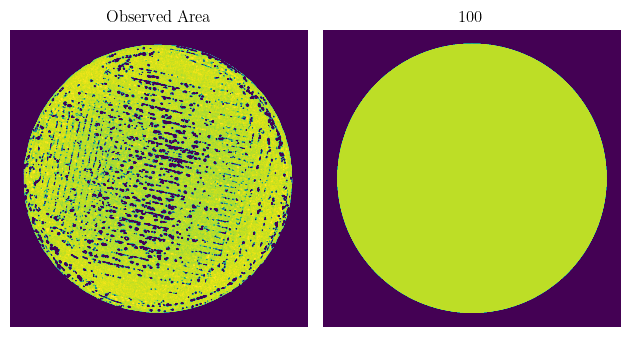
\includegraphics[width=0.75\textwidth]{circle_mask.png}
        \caption{\emph{Two images showing the observed data of the cross-section, after thresholding, and the scaled circle mask generated using prior knowledge from the dimensioning task.}}
    \end{figure}

\subsection{Segmentation}
    \subsubsection{Histogram Analysis}
        The simplest approach to segmentation is to simply look at the histogram of intensities measured in the volume. This histogram is seen in Figure \ref{fig:histogram} and demonstrates a key issue with this method.

        \begin{figure}[H]
            \centering
            \label{fig:histogram}
            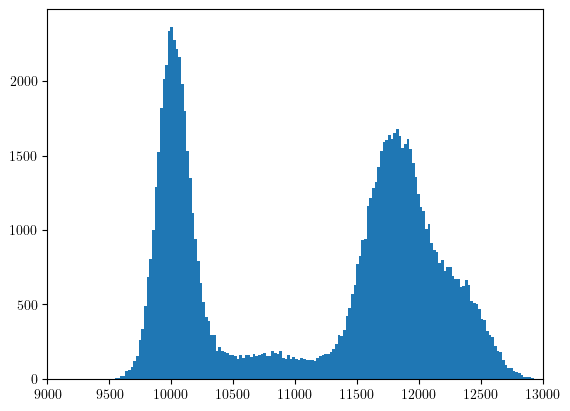
\includegraphics[width=0.75\textwidth]{histogram.png}
            \caption{\emph{The histogram of a uniform random sampling of intensities throughout the volume. Notice how even though there are three distinct materials, and the background, there are not distinct peaks to match.}}
        \end{figure}

        The range of intensities observed for each material  overlap much too closely to be able to distinguish regions just from it alone.

    \subsubsection{Gaussian Mixture Model}
        Knowing that the histogram can't be easily differentiate manually, we decided to apply a well-defined method to this task. Using Scikit-learn, we created a Gaussian Mixture Model using our data as input. This works well to determine the component Gaussian distributions that are present, allowing us to isolate means for each material and the standard deviation of each. There was some uncertainty as to how many distributions were actually present, so the models are shown in Figure \ref{fig:GMM}.

        \begin{figure}[H]
            \centering
            \label{fig:GMM}
            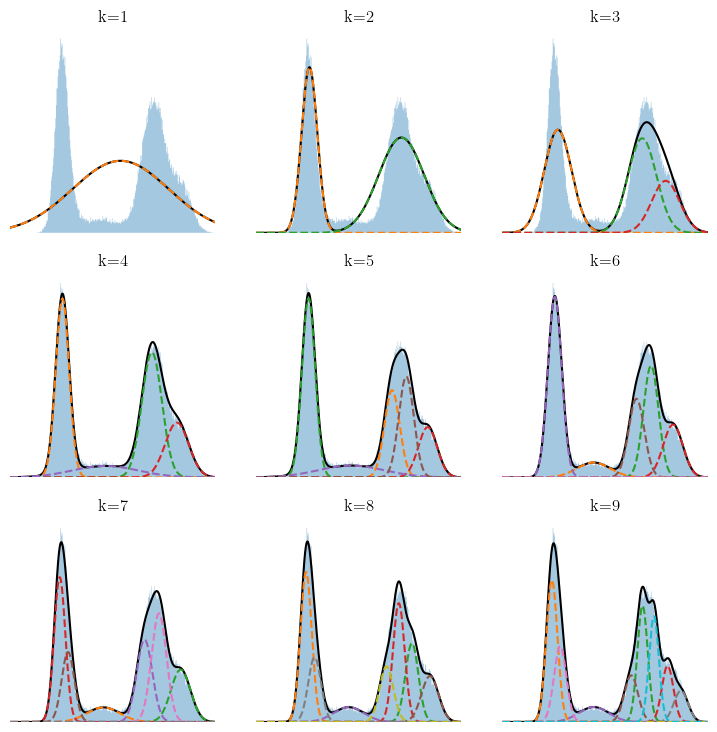
\includegraphics[width=0.85\textwidth]{GMM.png}
            \caption{\emph{A grid of plots showing the histogram of the dataset and the k best-fit Gaussian distributions for it.}}
        \end{figure}

        This method did not succeed in segmenting the data on its own, but it provided useful data and knowledge that was applied towards all following methods.

    \subsubsection{Region-Growing}
        After further research into 3-D segmentation, we came across region-growing as a commonly used method. This method involves user-provided seed values with known material tags. The algorithm then explores outward from these points following predefined rules. Based on the outcome of these rules, the material of the surrounding voxels are determined. This algorithm was extremely effective on 2-D tests, as seen in Figure \ref{fig:region-growing}, but was far too complex for us to efficiently implement in 3-D.

        \begin{figure}[H]
            \centering
            \label{fig:region-growing}
            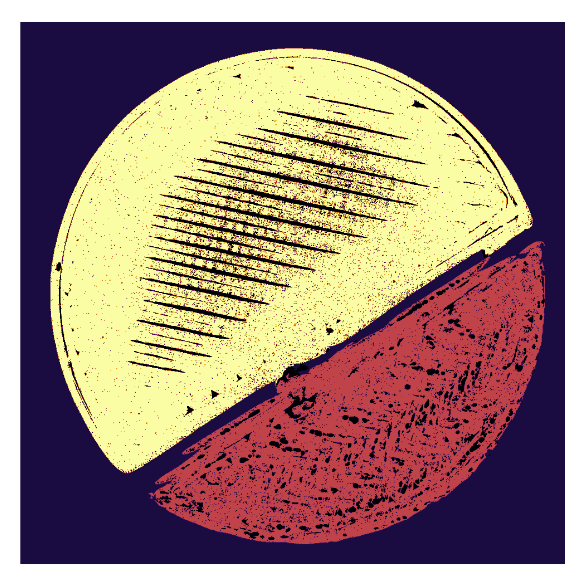
\includegraphics[width=0.5\textwidth]{region-growing.png}
            \caption{\emph{An example of a region-growing output on a 2-D slice of the volume.}}
        \end{figure}

    \subsubsection{Third-Party Tools}
        Due to the failures of the other methods, we began to explore third-party tools that are capable of segmentation. Early on, MATLAB was tried but very quickly abandoned due to performance and stability issues. It was easy to use though.

        3D Slicer was attempted to no avail.

        Insight Toolkit (ITK), a widely-used medical imaging library which we often have used for data visualization, has extensive segmentation support. Unfortunately these features have little-to-no documentation, making testing and development extremely slow and behind schedule. After many crashed sessions, only one complete run was performed, and the data was unusable. ITK was abandoned.

        The final third-party tool attempted is Drishti. This is a joint project between several Indian and Australian universities to create better CT segmentation and rendering tools for archaeology. The tool seems to have much potential, and was able to handle our dataset with ease. Unfortunately it suffers from the same issues as ITK when it comes to documentation. After many hours were dumped into attempting to learn this tool, it was also abandoned.

    \subsubsection{Manual Separation}
        The final attempted method is very manual in nature. It requires a large amount of work from the user. Seeing as other methods failed due to the similarity of materials being too close to each other, we decided to isolate regions of the image where the differences were far greater. This resulted in three tensors which contained each respective material and the background exclusively. Two other tensors were created containing only the boundary regions within the print.

        The test article was separated from the background in each of the three isolated tensors by simply thresholding the values to remove the background. This process is extremely quick to perform.

        Handling of the boundary regions is done through manual estimation of the bounding plane. We manually looked through slices of the volume in these regions to define three distinct points. These points were combined to define the plane which separates the materials. Each point in the isolated volume was evaluated to be above or below this plane, and the material was assigned based on the outcome. These materials were separated from the background using thresholding as previously performed.

\section{Results}
\subsection{Dimensioning}
    Each diameter measuring method arrived upon diameters of almost exactly 2 centimeters, which matches the CAD file defining the object. The masking method was completed without accounting for uncertainty, and had an output of simply 1.999 centimeters. The Hough circle transform properly handled uncertainty and provided a range of values the diameter falls within of 1.8394 to 2.2482 centimeters. The diameter measured throughout the object via masking is shown within Figure \ref{fig:diameter}.

    \begin{figure}[H]
        \centering
        \label{fig:diameter}
        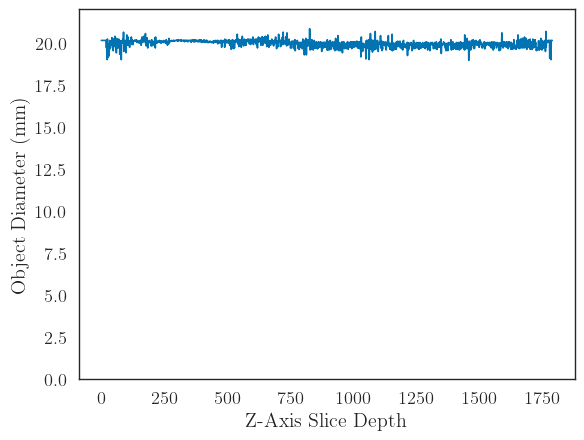
\includegraphics[width=0.75\textwidth]{diameters.png}
        \caption{\emph{The diameter of the test article as measured at each slice through the volume.}}
    \end{figure}

    The height dimensioning method returned a height of 3.55 centimeters, near what was expected. The visual analysis via 3D slicer matched this as well.

\subsection{Infill Analysis}
\subsubsection{Grid Subdivision}
The following figure demonstrates the first successful result obtained from the implementation of this approach upon slice \#575:

\begin{figure}[H]
 \centering
 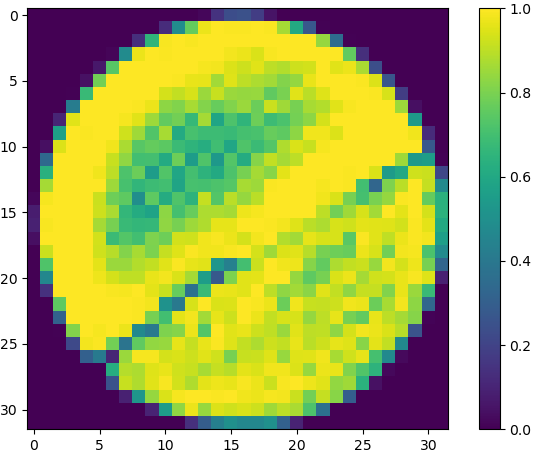
\includegraphics[width=0.65\textwidth]{images/575ratios.png}
 \caption{\textit{A colormap of the material-to-air ratios in Image Slice 575, with a threshold value of 100 and a gridscale value of 32. The image clearly shows darker regions of the slice, which represent more "airy" parts of the object's interior.}}
 \label{fig:575ratios}
\end{figure}

Additionally, the regions which do not meet the industry standard material-to-air ratio of 0.95 can be set to another arbitrary value (higher than zero but lower than 0.95) in order to highlight such regions.  This is done in the following figure, also for slice \#575:

\begin{figure}[H]
 \centering
 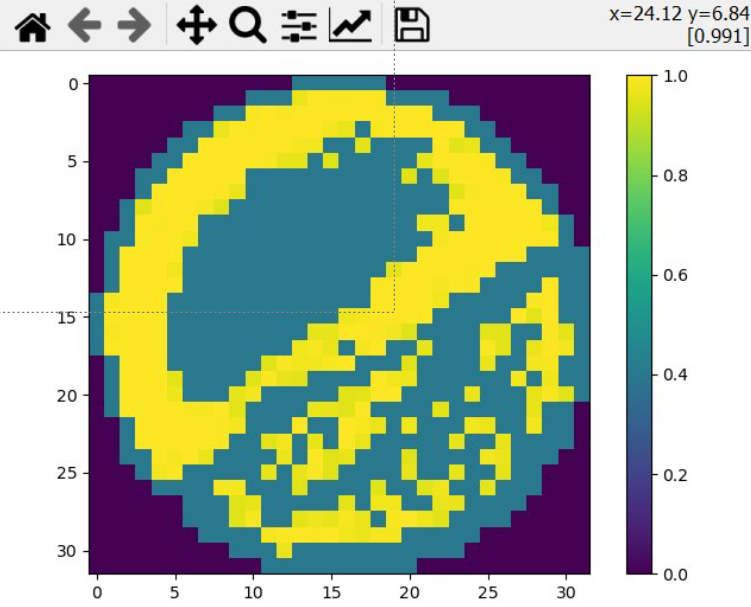
\includegraphics[width=0.65\textwidth]{images/underfill.png}
 \caption{\textit{A colormap of the material-to-air ratios in Image Slice 575, where regions with an infill ratio below 0.95 are assigned an arbitrary value so as to specifically highlight regions within the slice which do not meet the industry infill standards.}}
\end{figure}

Based on the distribution of infill ratios within this slice, air pockets and other manufacturing anomalies which affect the interior material distribution are made clear.  The analytical process used to create the colormap of ratios for this particular slice can be applied to all other slices in the object as well; by changing the target slice, threshold value, and gridscale,  the capacity for infill analysis of this object using the Grid Subdivision approach is quite extensive. Additionally, this approach can be used for other 3-D printed objects for which CT data is available, making it an incredibly versatile vector of analysis for object interiors.

\subsubsection{Region-Filling}
Due to difficulties with implementing this method, no results have been completed as of writing this report.

\subsubsection{Mask Comparison}
The mask comparison was able to determine infill densities within all samples provided. The preparation of three test samples is highlighted within Figure \ref{fig:mask-comparison}.

\begin{figure}[H]
    \centering
    \label{fig:mask-comparison}
    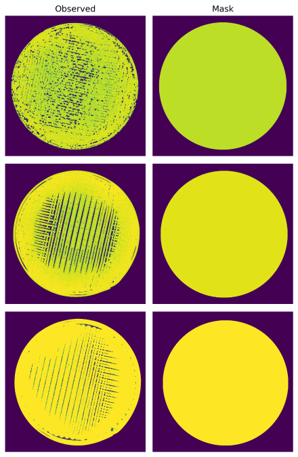
\includegraphics[width=0.75\textwidth]{mask_comparison.png}
    \caption{\emph{A grid of images demonstrating the preparation of test cross-sections for infill analysis.}}
\end{figure}

Each material has a distinct difference in infill density, with the nylon printing at a 93.1\% infill density, the polycarbonate printing at 91.8\% infill density, and the PLA printing at 97.2\% infill density.

\subsection{Segmentation}
The manual separation segmentation method resulted in the following figures:

\begin{figure}[H]
    \centering
    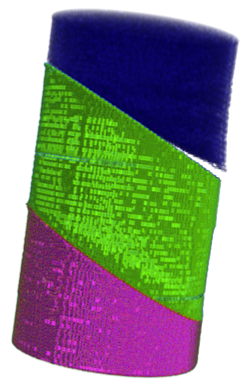
\includegraphics[width=0.35\textwidth]{ITK.png}
    \caption{\emph{A screenshot of 3-D visualization via ITK of the region segmentation performed by the manual separation.}}
\end{figure}

\begin{figure}[H]
    \centering
    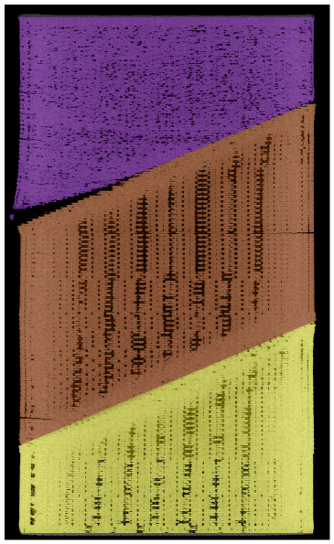
\includegraphics[width=0.4\textwidth]{manual-sep.png}
    \caption{\emph{A cross-section showing the segmentation throughout the entire sample.}}
\end{figure}

\section{Future Work}
\indent Infill Analysis: 
\begin{itemize}
    \item Infill analysis can be expanded to compare the print against Gcode. This can help quantify errors in the print.
\end{itemize}

Segmentation: 
\begin{itemize}
    \item Can be improved using machine learning and statistical approaches.
    \begin{itemize}
        \item This requires an annotated dataset of CT scans.
    \end{itemize}
    \item Improved segmentation may aid in defect detection and quantification.
    \item Region-growing may be applied near boundary regions to fix errors from plane division.
\end{itemize}

Defect Detection:
\begin{itemize}
    \item Using segmentation, defects can be found and highlighted, providing insight into the quality and usability of the component.
\end{itemize}

\section{References}
\printbibliography

\end{document}
